\section{General design description}\label{sec:general design}
This section describes the entire working of the system in an abstract way. The details of the concrete implementation can be found in Section \ref{sec:implementation}.

\ind The \ac{ips} consists of three main parts: the on site sensors and gateway, the frontend application and the backend. \\

The backend is the central entity in the system, as both the local system and the frontend application connect to it in order to query and post data. This is done via a \ac{rest} \ac{api}, which transfers data in a \ac{json}-format; the standard for \ac{rest} \acp{api} \cite{rest_apis}. The backend consists out of the combination of the servers which handle in the incoming requests and the database, which stores all the information about the parking garage (e.g. occupancy of parking lots, users inside the parking garage, etc.).
The backend also hosts the web variant of the frontend application and thus needs proper redirecting in order to redirect requests to the right destinations (in casu the frontend application or the database). The backend resides in a separate location (e.g. a data centre), separated from the actual garage. \\

The local setup requires a gateway  (\ac{iot}-device) and sensors installed in the physical garage. The sensors and the gateway are preferably connected through a \ac{lan}, but cable wiring is also possible, although less practical.

\ind The gateway is a micro-controller or \ac{iot}-device which is the central processing unit for the local system. When the local system exists out of multiple \ac{iot}-devices, an extra micro-controller can serve as a gateway for all these devices. This micro-controller can post and request data from the backend and controls the interaction between the different sensors. It performs only simple logical tasks, but delegates complex calculations to the backend.

\ind Two cameras detect entering and exiting cars, via \ac{anpr}. They are linked via the gateway with two servo motors, which control the barriers for entering and exiting the garage. Inside the garage, sensors detect if a parking lot is occupied or not. A \ac{led} visually indicates to the drivers if the parking lot is occupied/reserved. Furthermore, a display at the entrance of the garage indicates the amount of free spots left. \\

The frontend application serves as a \ac{gui} for the users to interact with the backend database. The application comes in two formats: a mobile application which is installable on both iOS and Android and a web application in the form of a website. Both variants have the same functionality. Figure \ref{fig:abstract-diagram} gives a very schematic overview of the different components of the \ac{ips}.\footnote{All figures and tables without an explicit credit are proprietary.}

\begin{figure}[htp]
    \centering
    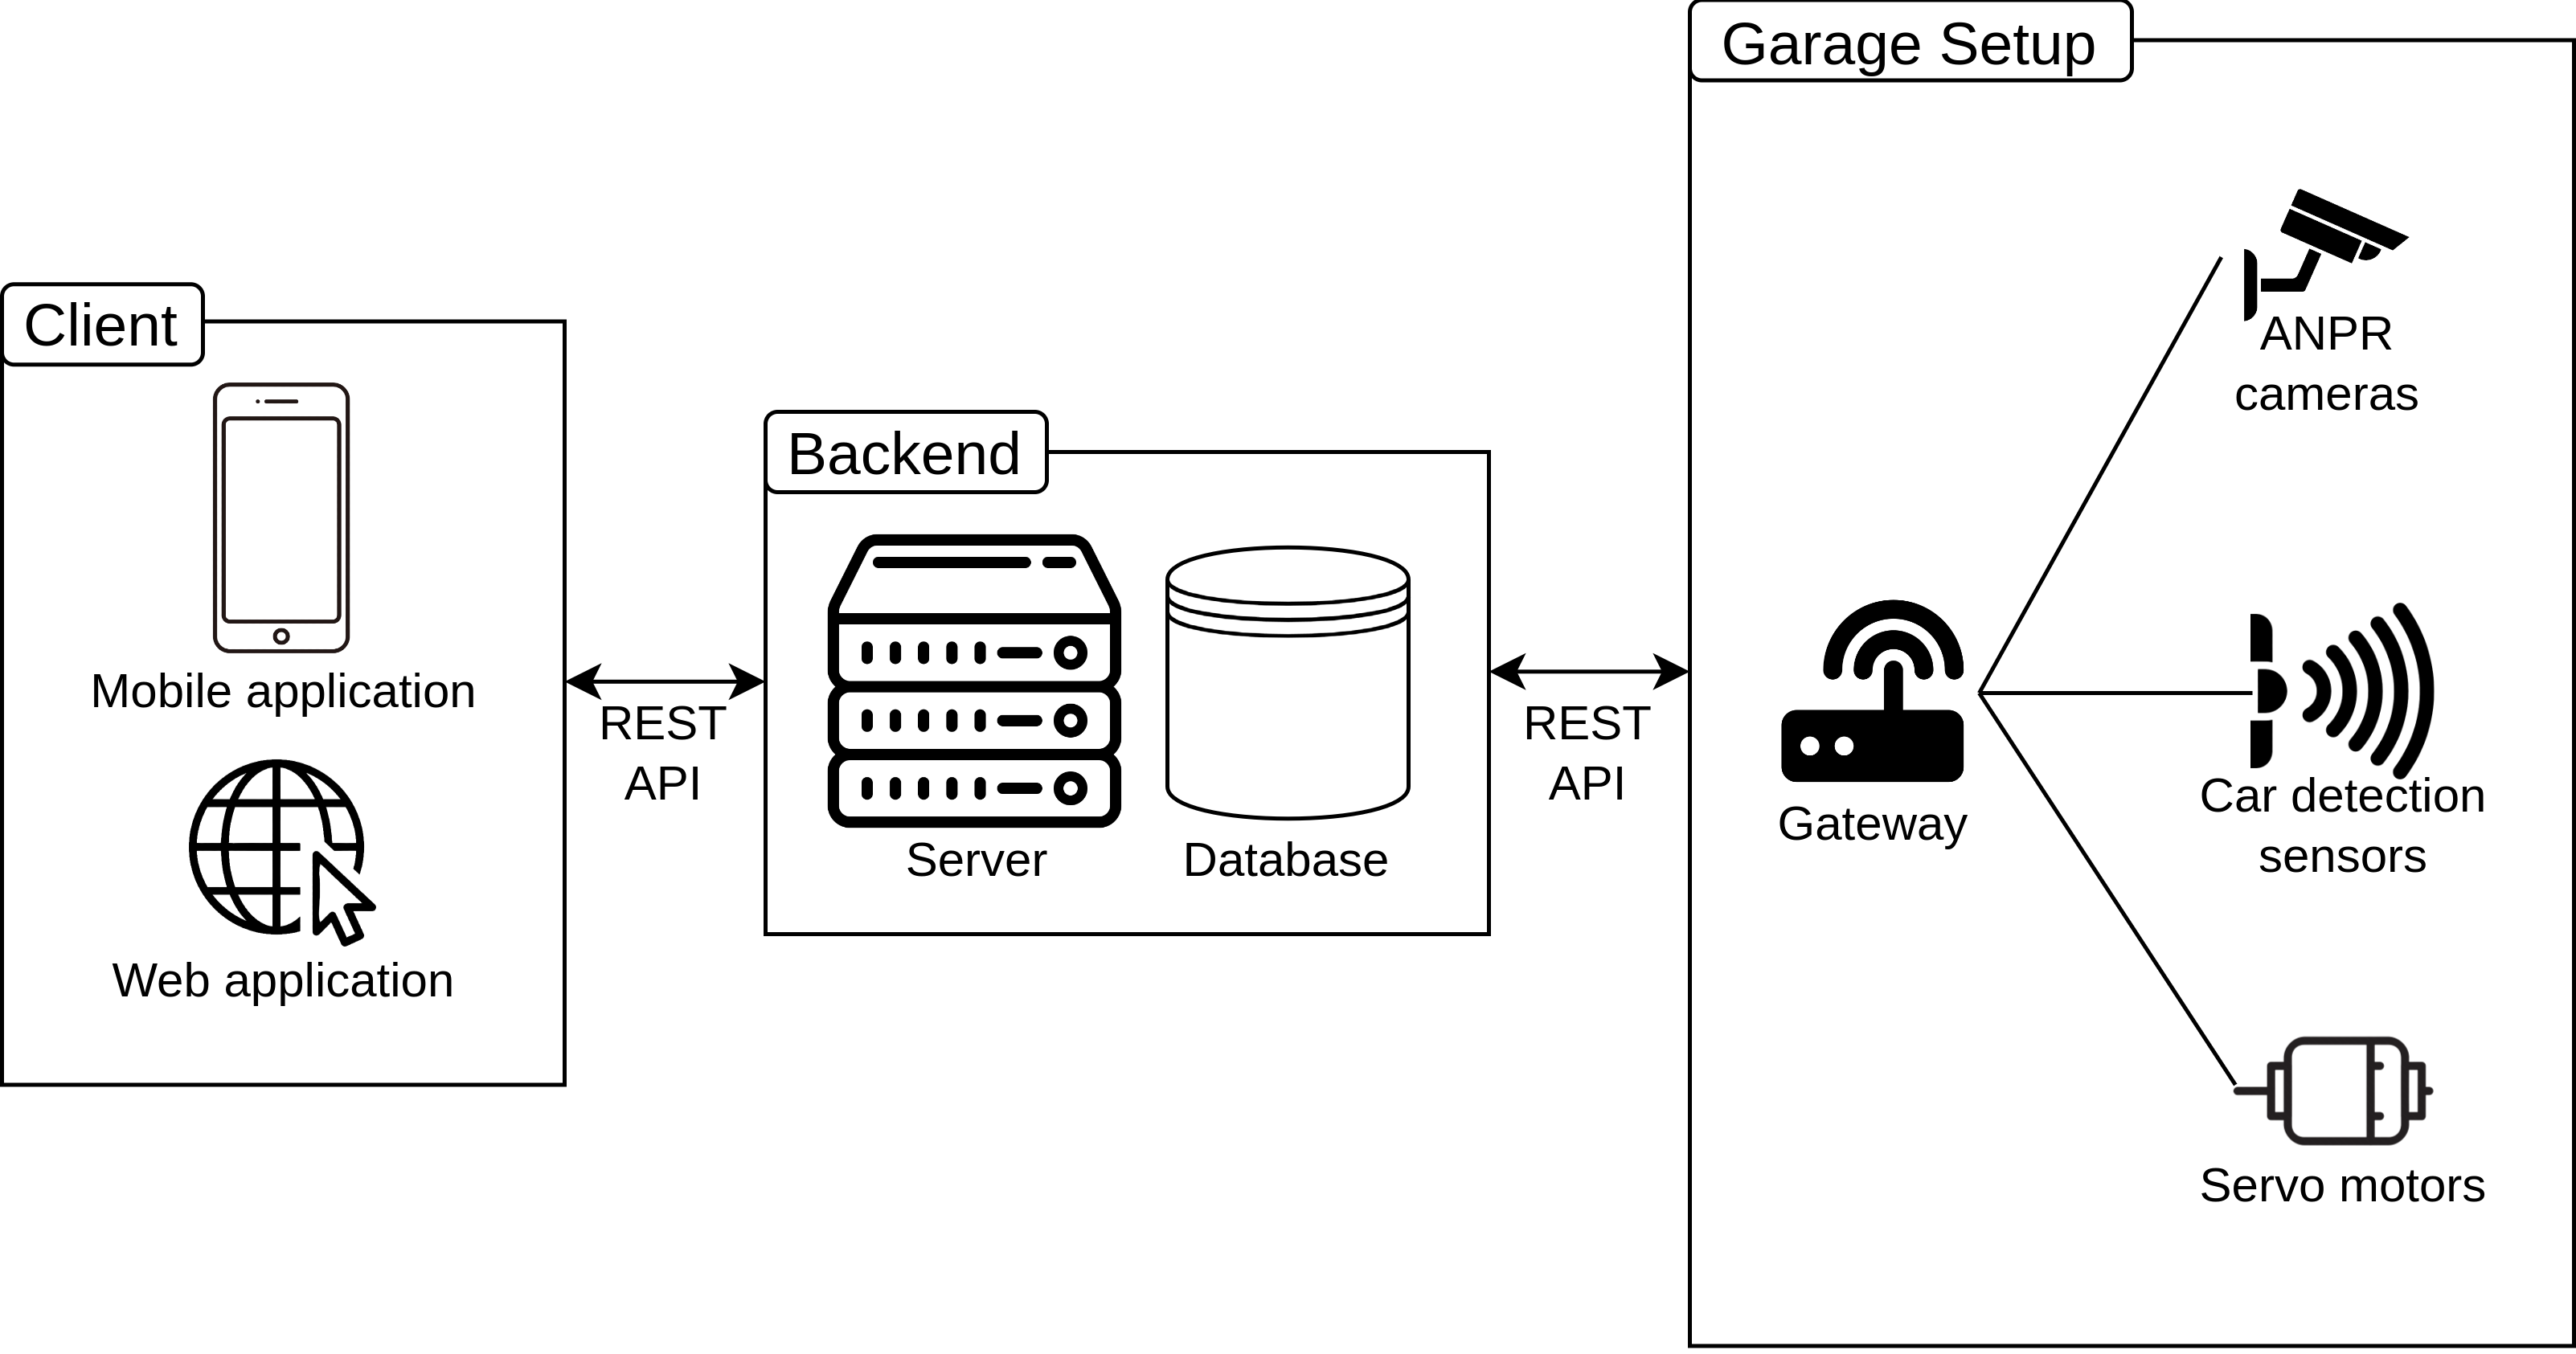
\includegraphics[width=12cm]{images/misc/abstract_diagram.drawio.png}
    \caption[Abstract overview of the intelligent parking system.]{Abstract overview of the intelligent parking system. The backend can be deployed on one psychical machine, which can run the proxy server and the database server in parallel.}
    \label{fig:abstract-diagram}
\end{figure}


\subsection{Core functionalities}\label{sec:core-functionalities}
The three main spearheads of the \ac{ips} described above are user privacy, security and ease of use. Table \ref{tab:core-functionalities} gives a summary of this paragraph, listing the three core functionalities, together with the steps taken to achieve them.
\ind Ease of use is split up in three sub-objectives.

\ind Firstly, it is not necessary for users of the parking garage to install the mobile application or even have a pre-existing account. It is possible for users to drive to the parking garage and park without any need for a prior setup, but receive an almost equal user experience.

\ind Secondly, if the user creates an account, he/she is able to reserve parking lots in a specific garage between specific times, in order to guarantee an available parking lot for the user at his/her arrival.

\ind Thirdly, the infrastructure supports automatic and non-automatic payments from within the frontend application, the former for users which created an account, the latter as an alternative for users without an account. 

\ind Besides the ease of use for the person parking in the garage, the frontend application also supports admin features for a garage owner. A garage owner can add or delete his/her garages from the system, as well as configure their parking lots. \\

Maximum user privacy is achieved by, firstly, not storing any information that is not needed for the operation of the \ac{ips} and secondly, hashing all user-identifiable and/or sensitive information (e.g. passwords, licence plates, email addresses) before it is stored inside the database. This way, even if an attacker obtains access to the database, he/she will not be able to retrieve any useful information from it.

\ind The two ways to park in the garage (i.e. with or without a pre-existing account) provide two levels of user privacy. If the user decides to park without an account, no user-identifiable information is stored in the database, except for the licence plate, which is deleted upon exit of the garage. This way, it is not possible to retrieve any personal information, nor information about the user's whereabouts from the system. From the standpoint of the system, that user ceases to exist upon exit of the garage. In the other case, licence plate information is coupled with the user's email address and a real first and last name, but history of the user's whereabouts are not stored (they are deleted upon exit of the garage).

\ind Making an automatic payment requires payment information from the user. This information is hashed before it is stored inside the database, but the user can opt for a manual payment, in which case no payment details are stored in the database.

\ind Furthermore, a garage owner is not able to query the users or licence plates in its garage, only the amount free parking lots left. \\ 

Security is the last core functionality. This mainly focuses on securing the backend, because it stores all important user information, but also includes securing the mobile application and the local garage setup, such that the sensors, nor the \ac{anpr}-cameras can be hijacked. 

\ind Firstly, the connections between the frontend and the backend and between the backend and the local garage gateway are encrypted. Secondly, the server only accepts traffic coming from the local garage gateway or the mobile application, which prevents \ac{csrf}-attacks. Thirdly, users can only query information regarding their own account (i.e. their personal information and bookings), which prevents \ac{idor}-attacks and fourthly, the \ac{api} can only be queried by authenticated users.

\begin{table}[htp]
    \centering
    \caption{An overview of the core functionalities of the entire system and how this is achieved on an abstract level.}
    \begin{tabular}{|>{\bfseries\centering\arraybackslash}m{1in}|>{\centering\arraybackslash}m{8cm}|}
         \hline
         \textbf{Core functionality} & \textbf{Achieved by}  \\
         \hline
         \hline
         Ease of use & \begin{itemize}[left=0pt]
             \item No obligatory account
             \item Reserving parking lots
             \item Automatic and non-automatic payments
             \item One application for both user and garage owners
         \end{itemize} \\
         \hline
         User privacy & \begin{itemize}[left=0pt]
             \item Least to know principle
             \item Hashing sensitive user information
         \end{itemize}\\
         \hline
         Security &\begin{itemize}[left=0pt]
             \item Encrypted connections
             \item Request origin validation
             \item Authenticated \ac{api}
         \end{itemize} \\
         \hline
    \end{tabular}
    \label{tab:core-functionalities}
\end{table}
